\documentclass[a4paper]{article}
%% Sets page size and margins
\usepackage[a4paper,top=3cm,bottom=3cm,left=3cm,right=3cm,marginparwidth=1.75cm]{geometry}
%% Useful packages
\usepackage{amsmath,amsthm,amssymb,amsfonts}
\usepackage{graphicx}
\usepackage[colorinlistoftodos]{todonotes}
\usepackage{bbm}
\usepackage{setspace}
\usepackage{footmisc}
\usepackage{pdflscape}
\usepackage{natbib}
\usepackage{booktabs}
\usepackage{caption}
\usepackage{subcaption}
\usepackage{changepage}
\usepackage{rotating}
\usepackage{bm}
\usepackage{tikz}
\usetikzlibrary{fit,tikzmark}  
\usetikzlibrary{shapes.geometric, arrows}
\usepackage{color, colortbl}

\usepackage{graphicx}
\usepackage[colorlinks=true, allcolors=blue]{hyperref}
\usepackage{url}

\renewcommand\footnotelayout{\fontsize{10}{12}\selectfont}


\tikzstyle{start} = [rectangle, rounded corners, 
minimum width=3cm, 
minimum height=1cm,
text centered, 
draw=black, 
fill=orange!30]

\tikzstyle{process} = [rectangle, 
minimum width=3cm, 
minimum height=1cm, 
text centered, 
text width=3cm, 
draw=black, 
fill=blue!30]

\tikzstyle{stop} = [rectangle, rounded corners, 
minimum width=3cm, 
minimum height=1cm,
text centered, 
draw=black, 
fill=green!30]

\tikzstyle{arrow} = [thick,->,>=stealth]



\interfootnotelinepenalty=10000

\newcommand{\R}{\mathbb{R}}
\newcommand{\N}{\mathbb{N}}
\newcommand{\Z}{\mathbb{Z}}
\providecommand{\C}{\mathbb{C}}

\theoremstyle{definition}
\newtheorem{defin}{Definição}

\theoremstyle{plain}
\newtheorem{theorem}[defin]{Teorema}
\newtheorem{corollary}[defin]{Corolário}

\linespread{2}
\title{Rawls For Electricity Planning Models}

\author{Lauren Beatty\thanks{Environmental Defense Fund  \hspace{.5cm} E-mail: lbeatty1@edf.org \hspace{.5cm}Website: \href{https://lbeatty1.github.io}{https://lbeatty1.github.io}}\\
Matthias Fripp\thanks{Energy Innovations}}

\date{\today}

\begin{document}
\maketitle
\begin{center}
    PRELIMINARY DRAFT - PLEASE DO NOT CITE OR DISTRIBUTE
\end{center}

\begin{abstract}
Renewed interest in the distributional impacts of policies require going beyond typical methods of analysis such as benefit-cost analysis.  In this paper we show how to use least-cost electricity planning models to design equitable systems by modifying their objective functions.  Rather than using the models to minimize costs, we provide the model with a min-max objective function on the distributional health effects of electricity generation and subject the solution to a total cost constraint.  This method provides a menu of plans that equitably reduce pollution exposure.
\end{abstract}


\newpage
\section{Introduction}
Climate change mitigation requires deep cuts to greenhouse gas emissions from the electricity sector.  Least-cost electricity planning models are powerful tools that help policymakers and capacity planners find portfolios of generation technologies that meet reliability requirements and emissions goals.  

However, these models have historically ignored some of the external costs of electricity generation. One major external costs is the generation of local air pollutants.  There is a large body of work on the health effects of air pollution, as well as a large body of work on the effects of electricity generation on air pollution. 
Air pollution is linked with numerous health impacts such as chronic obstructive pulmonary disease (COPD), acute lower respiratory illness, cerebrovascular disease, ischaemic heart disease, and lung cancer. \cite{Lelieveld2015TheScale} estimate that power generation is linked with 31$\%$ of premature mortality caused by outdoor air pollution in the U.S.

There is also work that has shown that air pollution exposures vary drastically across racial and socioeconomic groups.   \cite{Thind2019FineGeography} find that Black and non-Hispanic white people are exposed to more pollution than other groups and that exposures for low-income people are higher than for high-income people, even after controlling for race.  This highlights the importance of developing planning methods that alleviate rather than reinforce disproportionate burdens.

Previous work has included co-benefits involved with reducing electricity generation from fossil fuels in the objective function \citet{Sergi2020OptimizingBenefits}.
or projected how the electricity transmission might affect the distributional consequences of air pollution exposure \citep{Goforth2022AirStrategies}. 

Least-cost electricity planning models are the gold standard models used to model capacity expansion in policy.  However, these models tend to have a narrow focus on minimizing costs -- potentially at the expense of distributional concerns.  The energy transition will have wide-ranging effects --such as shifts in the spatial distribution of jobs, or changes in air pollution, that are of interest to policy-makers, but are currently unincorporated into least-cost models.

Previous attempts to consider the health impacts of air pollution have monetized air pollution harms, and inserted them into the cost minimization.  While this is certainly an improvement over not considering these costs at all, this method ignores the fact that inequity in the past has driven current differences in air pollution exposure, and that certain groups may experience higher burdens from air pollution than others.

However, in this paper, rather than modifying the objective function to include health effects, or use model outputs to project health changes, we endogenize pollution exposure within the electricity model in a way that explicitly considers distributional effects.  We pull inspiration from Rawls and formulate our model as a min-max problem where the social planner minimizes the maximum pollution exposure subject to a cost constraint, rather than minimizing costs.  Running multiple iterations of the model at different cost constraints allows us to understand how much can we equitably improve air quality and at what costs.

This allows us to use the model to produce results that don't unfairly burden certain groups with disproportionate pollution exposure.  It also can be used to answer questions such as "How much can pollution exposure be equitably reduced for $\$100$ billion?" 

This method could also be used to help design electricity transition plans that are equitable in other dimensions.  For example, one concern with the energy transition is that some regions will lose jobs.  This method could help policymakers and planners design electricity systems that avoid causing disruptive employment declines in certain regions. Previous work has linked declines in employment from  coal extraction to negative impacts such as decreases in home values, increases in poverty, and increases in credit utilization and delinquency. Moreover, these studies also suggest that even residents who are not employed by the industry also suffer the negatives consequences associated with the industry's decline (\citet{Kraynak2023TheCountry}, \citet{Blonz2023TheFuels}). 

This paper makes an important contribution to the environmental justice literature by endogenizing air pollution within a least-cost planning model, and proposing a framework to equitably reduce air pollution. Our findings indicate that major improvements to air pollution can be made with relatively small increases in overall cost.


\section{Data}
The fist task in our method is to construct emissions rates for sources in the model in tons per MWh. These emissions rates are constructed by combining emissions data from the U.S. Environmental Protection Agency (EPA), and generations data from the U.S. Energy Information Administration (EIA). We use the EPA-EIA Power Sector Data Crosswalk to merge generators across the two sources \citep{HuettemanEPA-EIACrosswalk}.

\subsection{Emissions Data}
Emissions data comes from two sources: EPA's Clean Air Markets Program Data (CAMD) and EPA's National Emissions Inventory (NEI).  The CAMD was created to track compliance with clean air programs, and thus, tracks emissions of CO$_2$, NO$_x$, and SO$_2$.  The NEI was created to track criteria pollutants, criteria precursors, and hazardous air pollutants from \textit{all} sources.  I get emissions of NH$_3$, VOC, and PM2.5 from the NEI.  Air pollution data is used to calculate source emissions rates in tons per MWh.

\subsection{Generation Data}
Data on the generation and location of existing plants comes from the EIA.


\subsection{Power Sector Modelling Inputs}
Stuff about PowerGenome?

\section{Methods}
\subsection{Overview}

\begin{figure}
    \begin{center}
        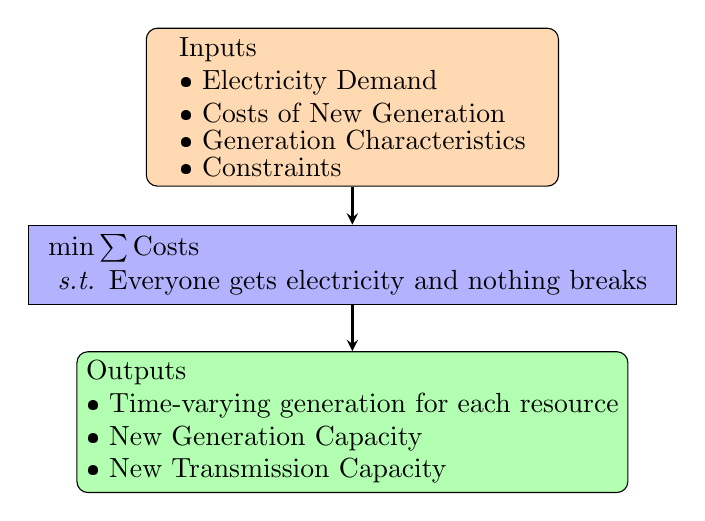
\begin{tikzpicture}[node distance=2cm]
        \node (start) [start, text width=5cm] {\shortstack[l]{Inputs\\• Electricity Demand \\ • Costs of New Generation \\ • Generation Characteristics\\
        • Constraints}};
        
        \node(obj)[process, below of=start, text width=8cm]{\shortstack[l]{$\min \sum \text{Costs}$ \\ \textit{ 
           s.t.   }\text{Everyone gets electricity and nothing breaks }}};
        
        \node (result) [stop, below of=obj] {\shortstack[l]{Outputs\\• Time-varying generation for each resource \\ • New Generation Capacity \\ • New Transmission Capacity}};
        
        \draw [arrow] (start) -- (obj);
        \draw [arrow] (obj) -- (result);
        
        \end{tikzpicture}
    \end{center}
    \caption{Typical Flow of Least-Cost Planning Models}
    \label{fig:enter-label}
\end{figure}


\begin{figure}
\begin{center}
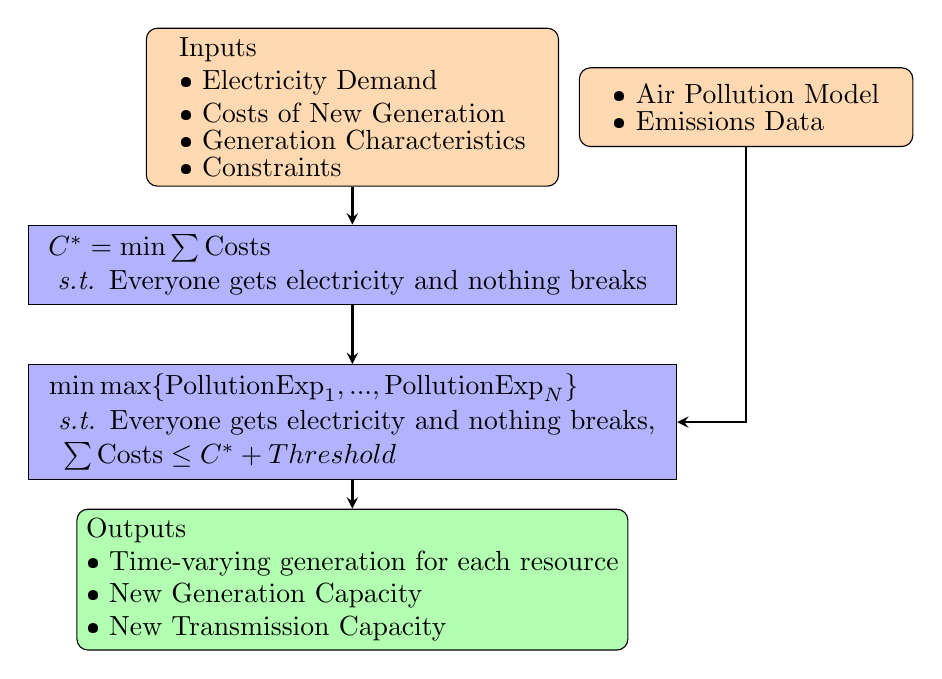
\begin{tikzpicture}[node distance=2cm]

\node (start) [start, text width=5cm] {\shortstack[l]{Inputs\\• Electricity Demand \\ • Costs of New Generation \\ • Generation Characteristics\\
• Constraints}};

\node (air) [start, text width=4cm, right of= start, xshift=3cm] {\shortstack[l]{• Air Pollution Model\\
• Emissions Data}};

\node(obj)[process, below of=start, text width=8cm, xshift=0cm]{\shortstack[l]{$C^* = \min \sum \text{Costs}$ \\ \textit{ 
   s.t.   }\text{Everyone gets electricity and nothing breaks }}};

\node(obj2)[process, below of=obj, text width=8cm, xshift=0cm]{\shortstack[l]{$\min \max\{\text{PollutionExp}_1,...,\text{PollutionExp}_N\}$ \\ \textit{ 
   s.t.   }\text{Everyone gets electricity and nothing breaks,} \\
    $\text{      }\sum \text{Costs} \leq C^*+Threshold$ }};

\node (result) [stop, below of=obj2] {\shortstack[l]{Outputs\\• Time-varying generation for each resource \\ • New Generation Capacity \\ • New Transmission Capacity}};

\draw [arrow] (start) -- (obj);
\draw [arrow] (air) |- (obj2);
\draw [arrow] (obj) -- (obj2);
\draw [arrow] (obj2) -- (result);


\end{tikzpicture}
\caption{Our Modification to the Least-Cost Planning Model}
\end{center}
\end{figure}

\subsection{Air Pollution Modelling}
The end product necessary to endogenize air pollution within electricity planning models are a set of coefficients that describe the marginal effect of a unit of electricity generation on population-weighted mean pollution exposure for different racial groups (though you could also apply the same logic and methodology to differing socio-economic groups more broadly, or more fine slices of the population to more closely approximate a true min-max).  

Eulerian chemical transportation models are computationally expensive and time consuming, so it's infeasible to embed this type of model within SWITCH.  Rather we use the InMAP Source-Receptor Matrix (ISRM) which is a reduced-form source-receptor matrix that describes the marginal effect of a unit of pollution on downwind concentrations of pollution exposure.

InMap itself is a reduced-form emissions-to-exposure model that uses annual-average parameters to reduce computation complexity relative to a time-resolved chemical transport model. InMap is designed to model annual average PM2.5 pollution exposure, and takes as inputs the annual emissions of volatile organic compounds (VOCs), nitrous oxides (NOx), ammonia (NH3), sulfur oxides (SOx), and primary PM2.5 \citep{Tessum2017InMAP:Interventions}.

The ISRM was developed to simplify InMAP even further \citep{Goodkind2019Fine-scaleEmissions}.  Initially, the ISRM was developed to describe the marginal damages from individual sources.  We simplify the ISRM even further by collapsing it so that, for each source, we save the marginal effect of one MWh of generation on \textit{population-weighted average exposure} by race.

\subsection{Switch}

\section{Results}
\subsection{Model Inputs}
There are a few findings from the construction of model inputs that are worth discussing. First, unsurprisingly, empirical data on emissions and generation reveals that coal is a dirty source of generation. However, when we translate emissions into marginal exposure coefficients, we find that the average relative difference between coal and natural gas decreases. In particular, it appears that natural gas plants are on average, closer to Asian and Latino population centers. A unit of electricity generated from coal only causes slightly more damage (in terms of population-weighted PM2.5 exposure) to Asians and Latinos than a unit of electricity generated from natural gas. In figure \ref{EmissionsExposureCoefs} we plot the average empirical emissions rates by technology in panel (a), and the mean coefficients describing how one MWh of generation affects mean group-level exposure of PM2.5 in $\mu$g/m$^3$. 

This start divergence between the relative emissions rates and the relative exposure coefficients highlights one of the central premises of the paper -- that where generation is placed can have large impacts on pollution exposure, and that selectively choosing what generation goes where can lead to large decreases in pollution exposure at low costs.

\begin{figure}
\centering
\subcaptionbox{Mean empirical emissions rates by technology in tons per MWh.}{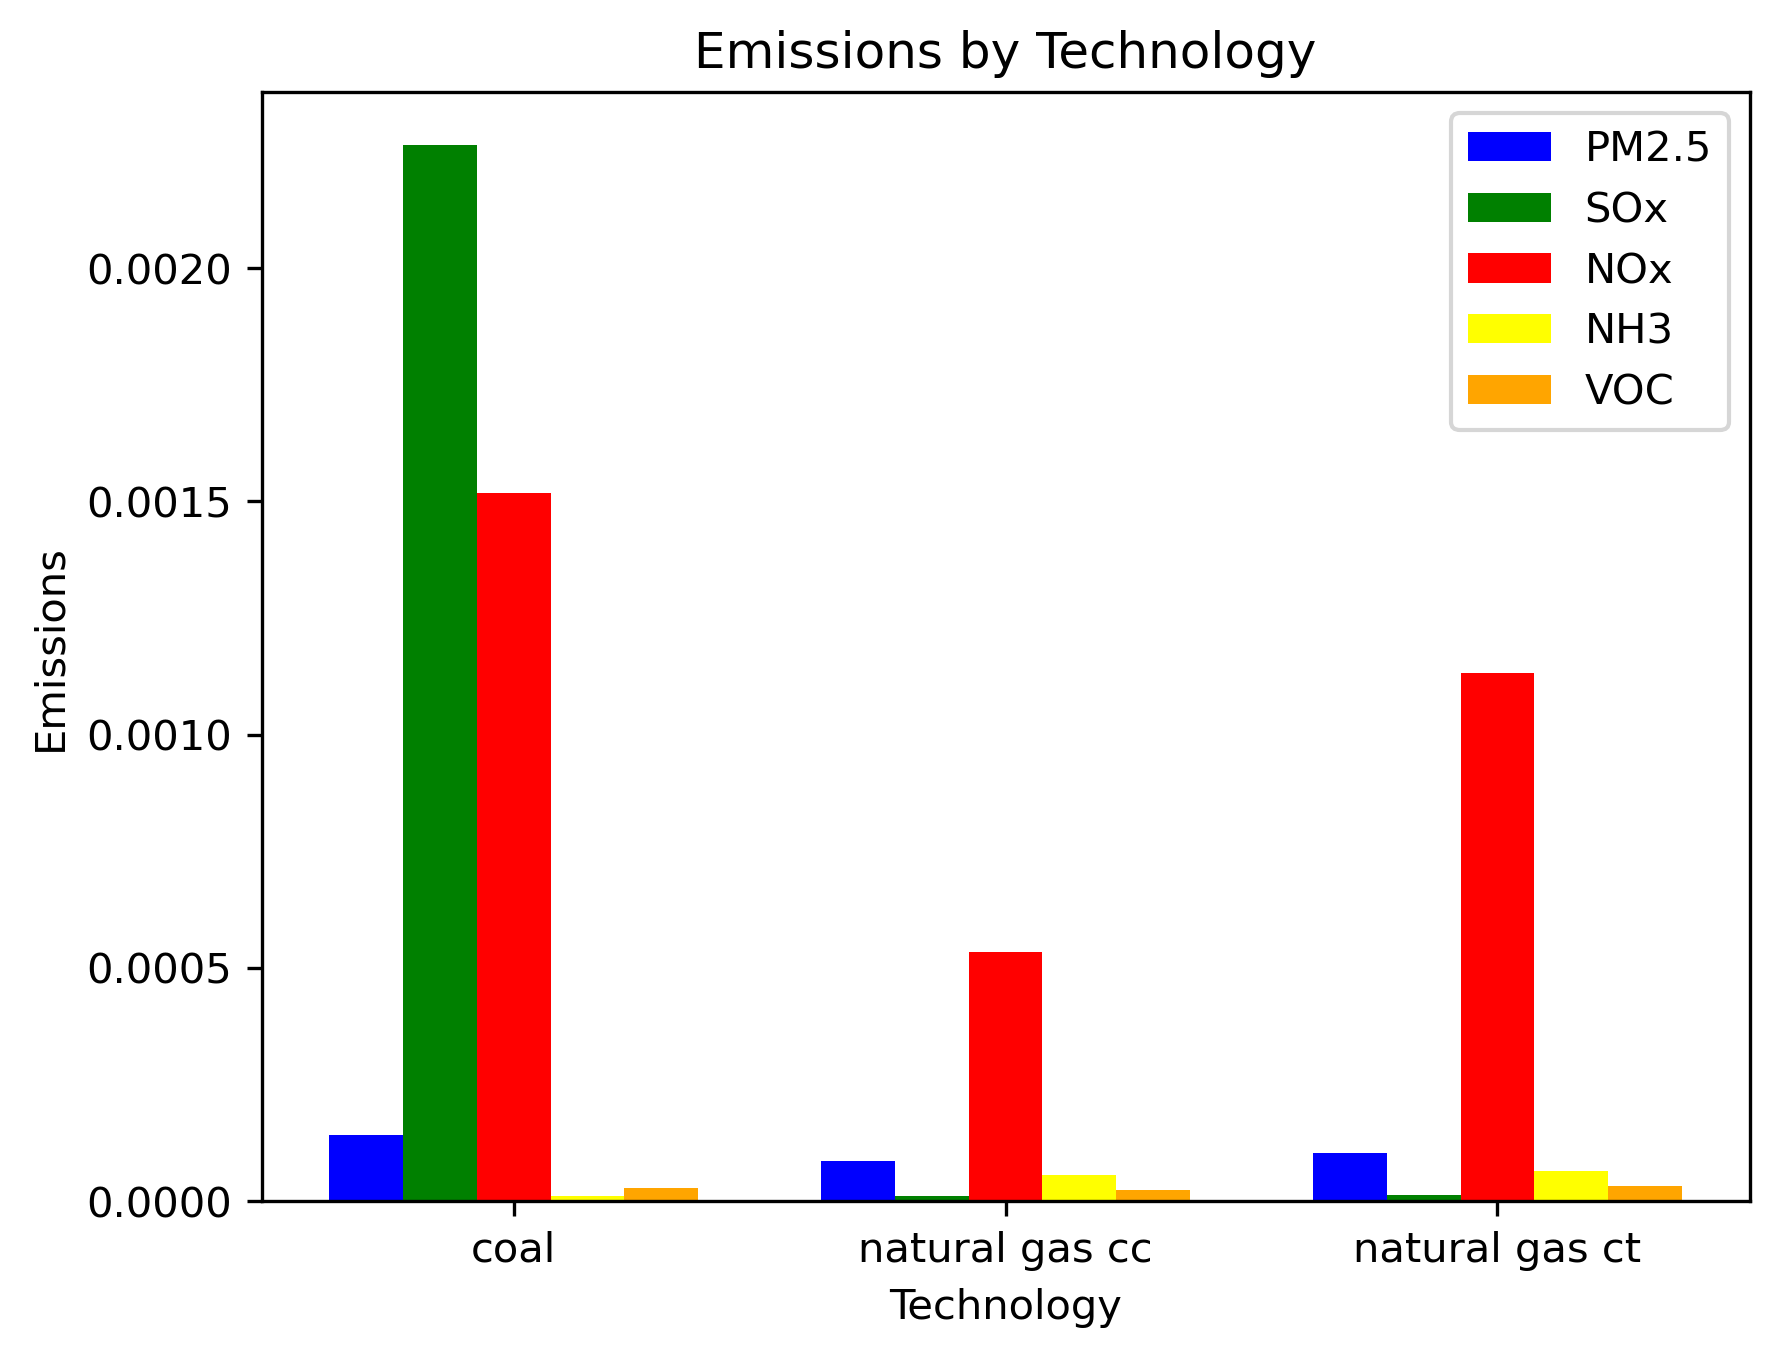
\includegraphics[width=0.45\textwidth]{Figures/EndogenousResults/base_short/base_short_emissions_by_technology.png}}%
\hfill
\subcaptionbox{Mean coefficients describing how a marginal MWh of generation affects mean group-level PM2.5 exposure.}{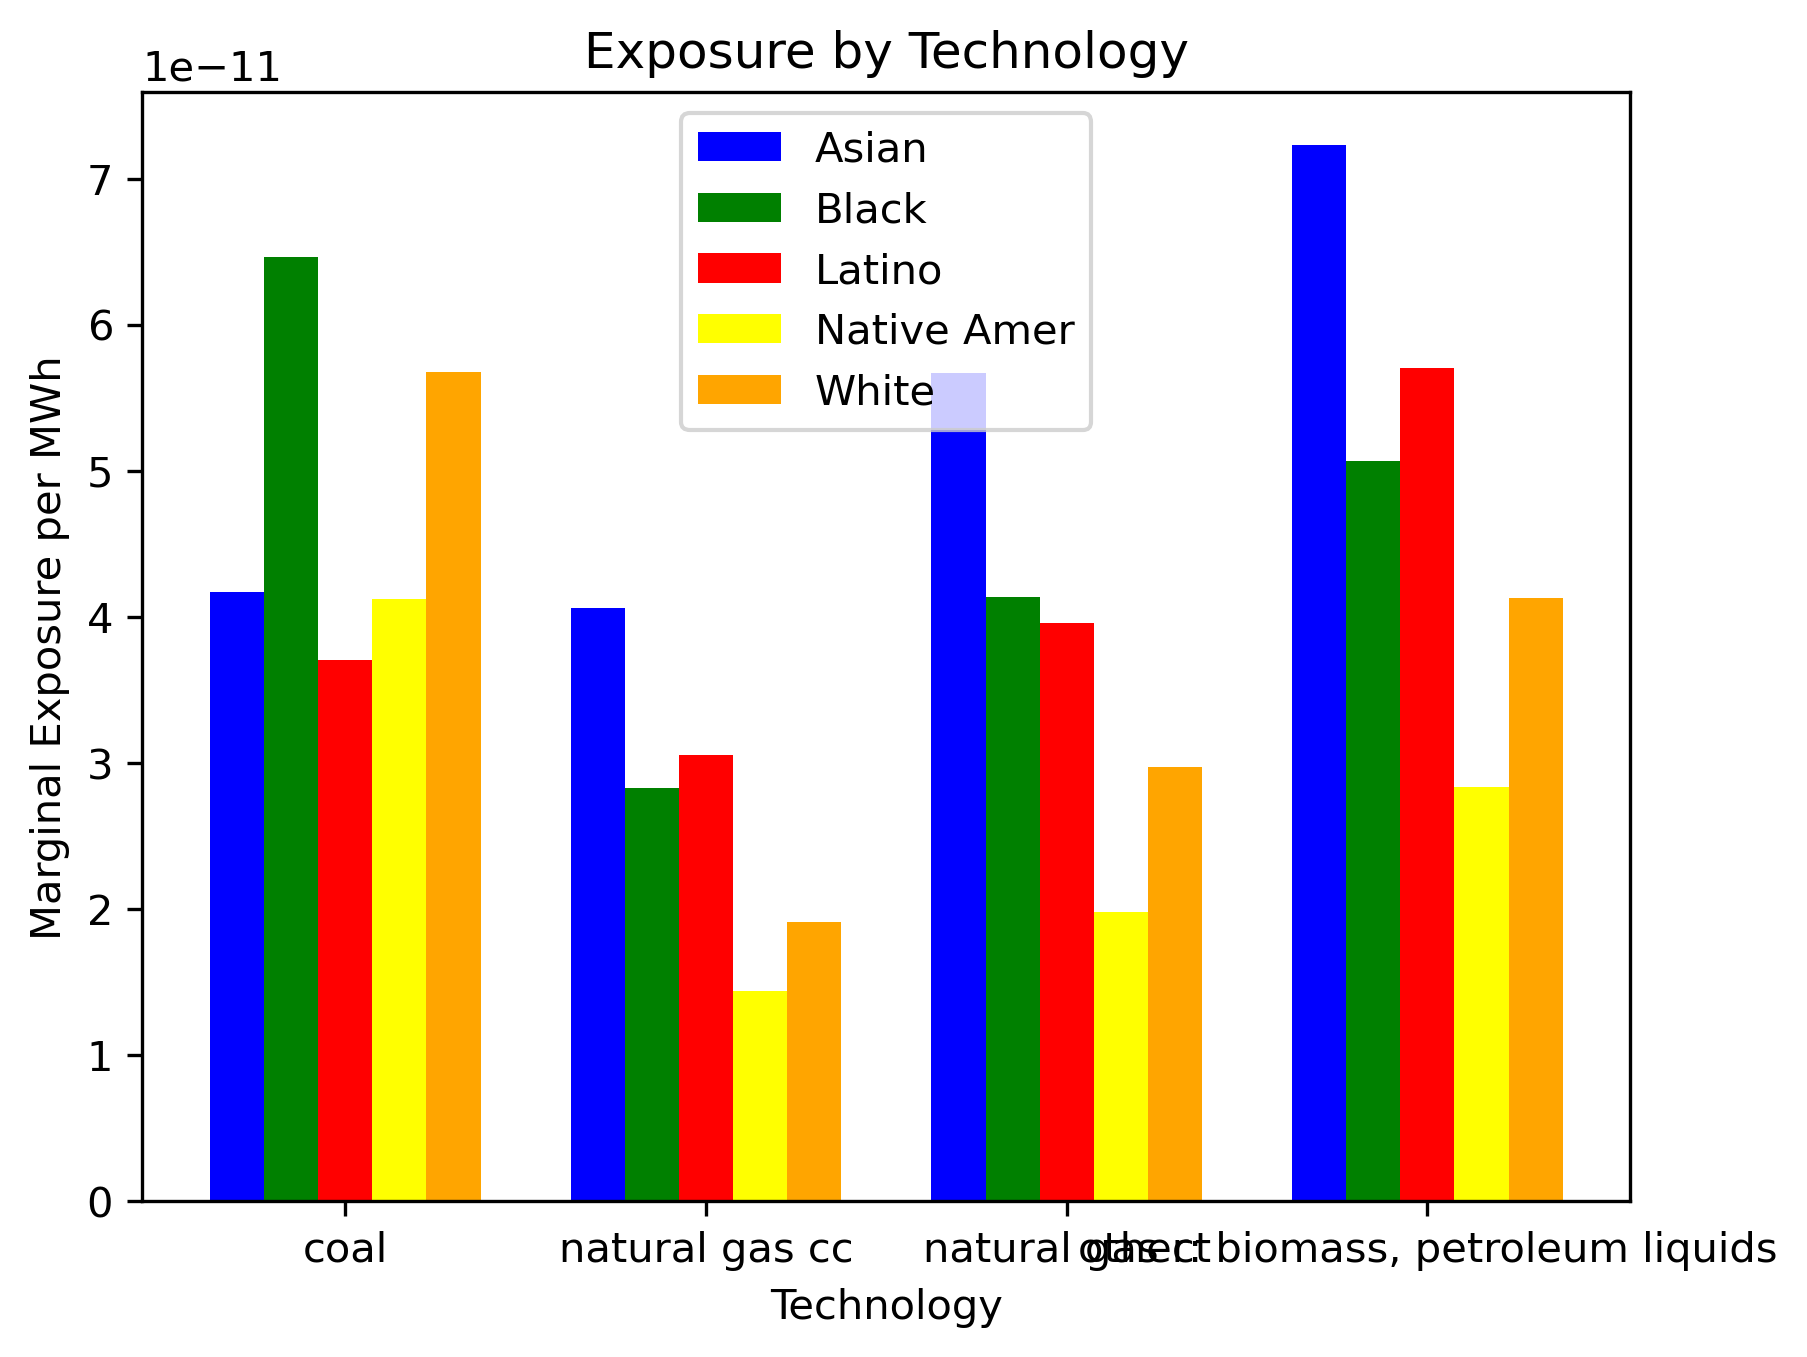
\includegraphics[width=0.45\textwidth]{Figures/EndogenousResults/base_short/base_short_exposure_by_technology.png}}%
\hfill
\caption{Unsurprisingly, coal is far dirtier than other technologies.  However, the discrepancy between technologies is more narrow for exposure.}
\label{EmissionsExposureCoefs}
\end{figure}

\subsection{Model Results}
Our high-level, key finding is that even a modest budget of $\$50$ billion through 2050 could pay for massive reductions in equitable air quality improvement. Our results have features that you would expect based on economic theory. There are increasing costs of reducing air pollution -- the gains from moving from least-cost to allocating $\$50$ billion are much larger than the gains from moving from allocating $\$50$ billion to $\$100$ billion. Our results also suggest that at the optimum, the min-max objective generates equal average exposures for all groups except Native Americans, who have consistently lower exposure levels.

\begin{figure}
    \centering
    \subcaptionbox{2027}{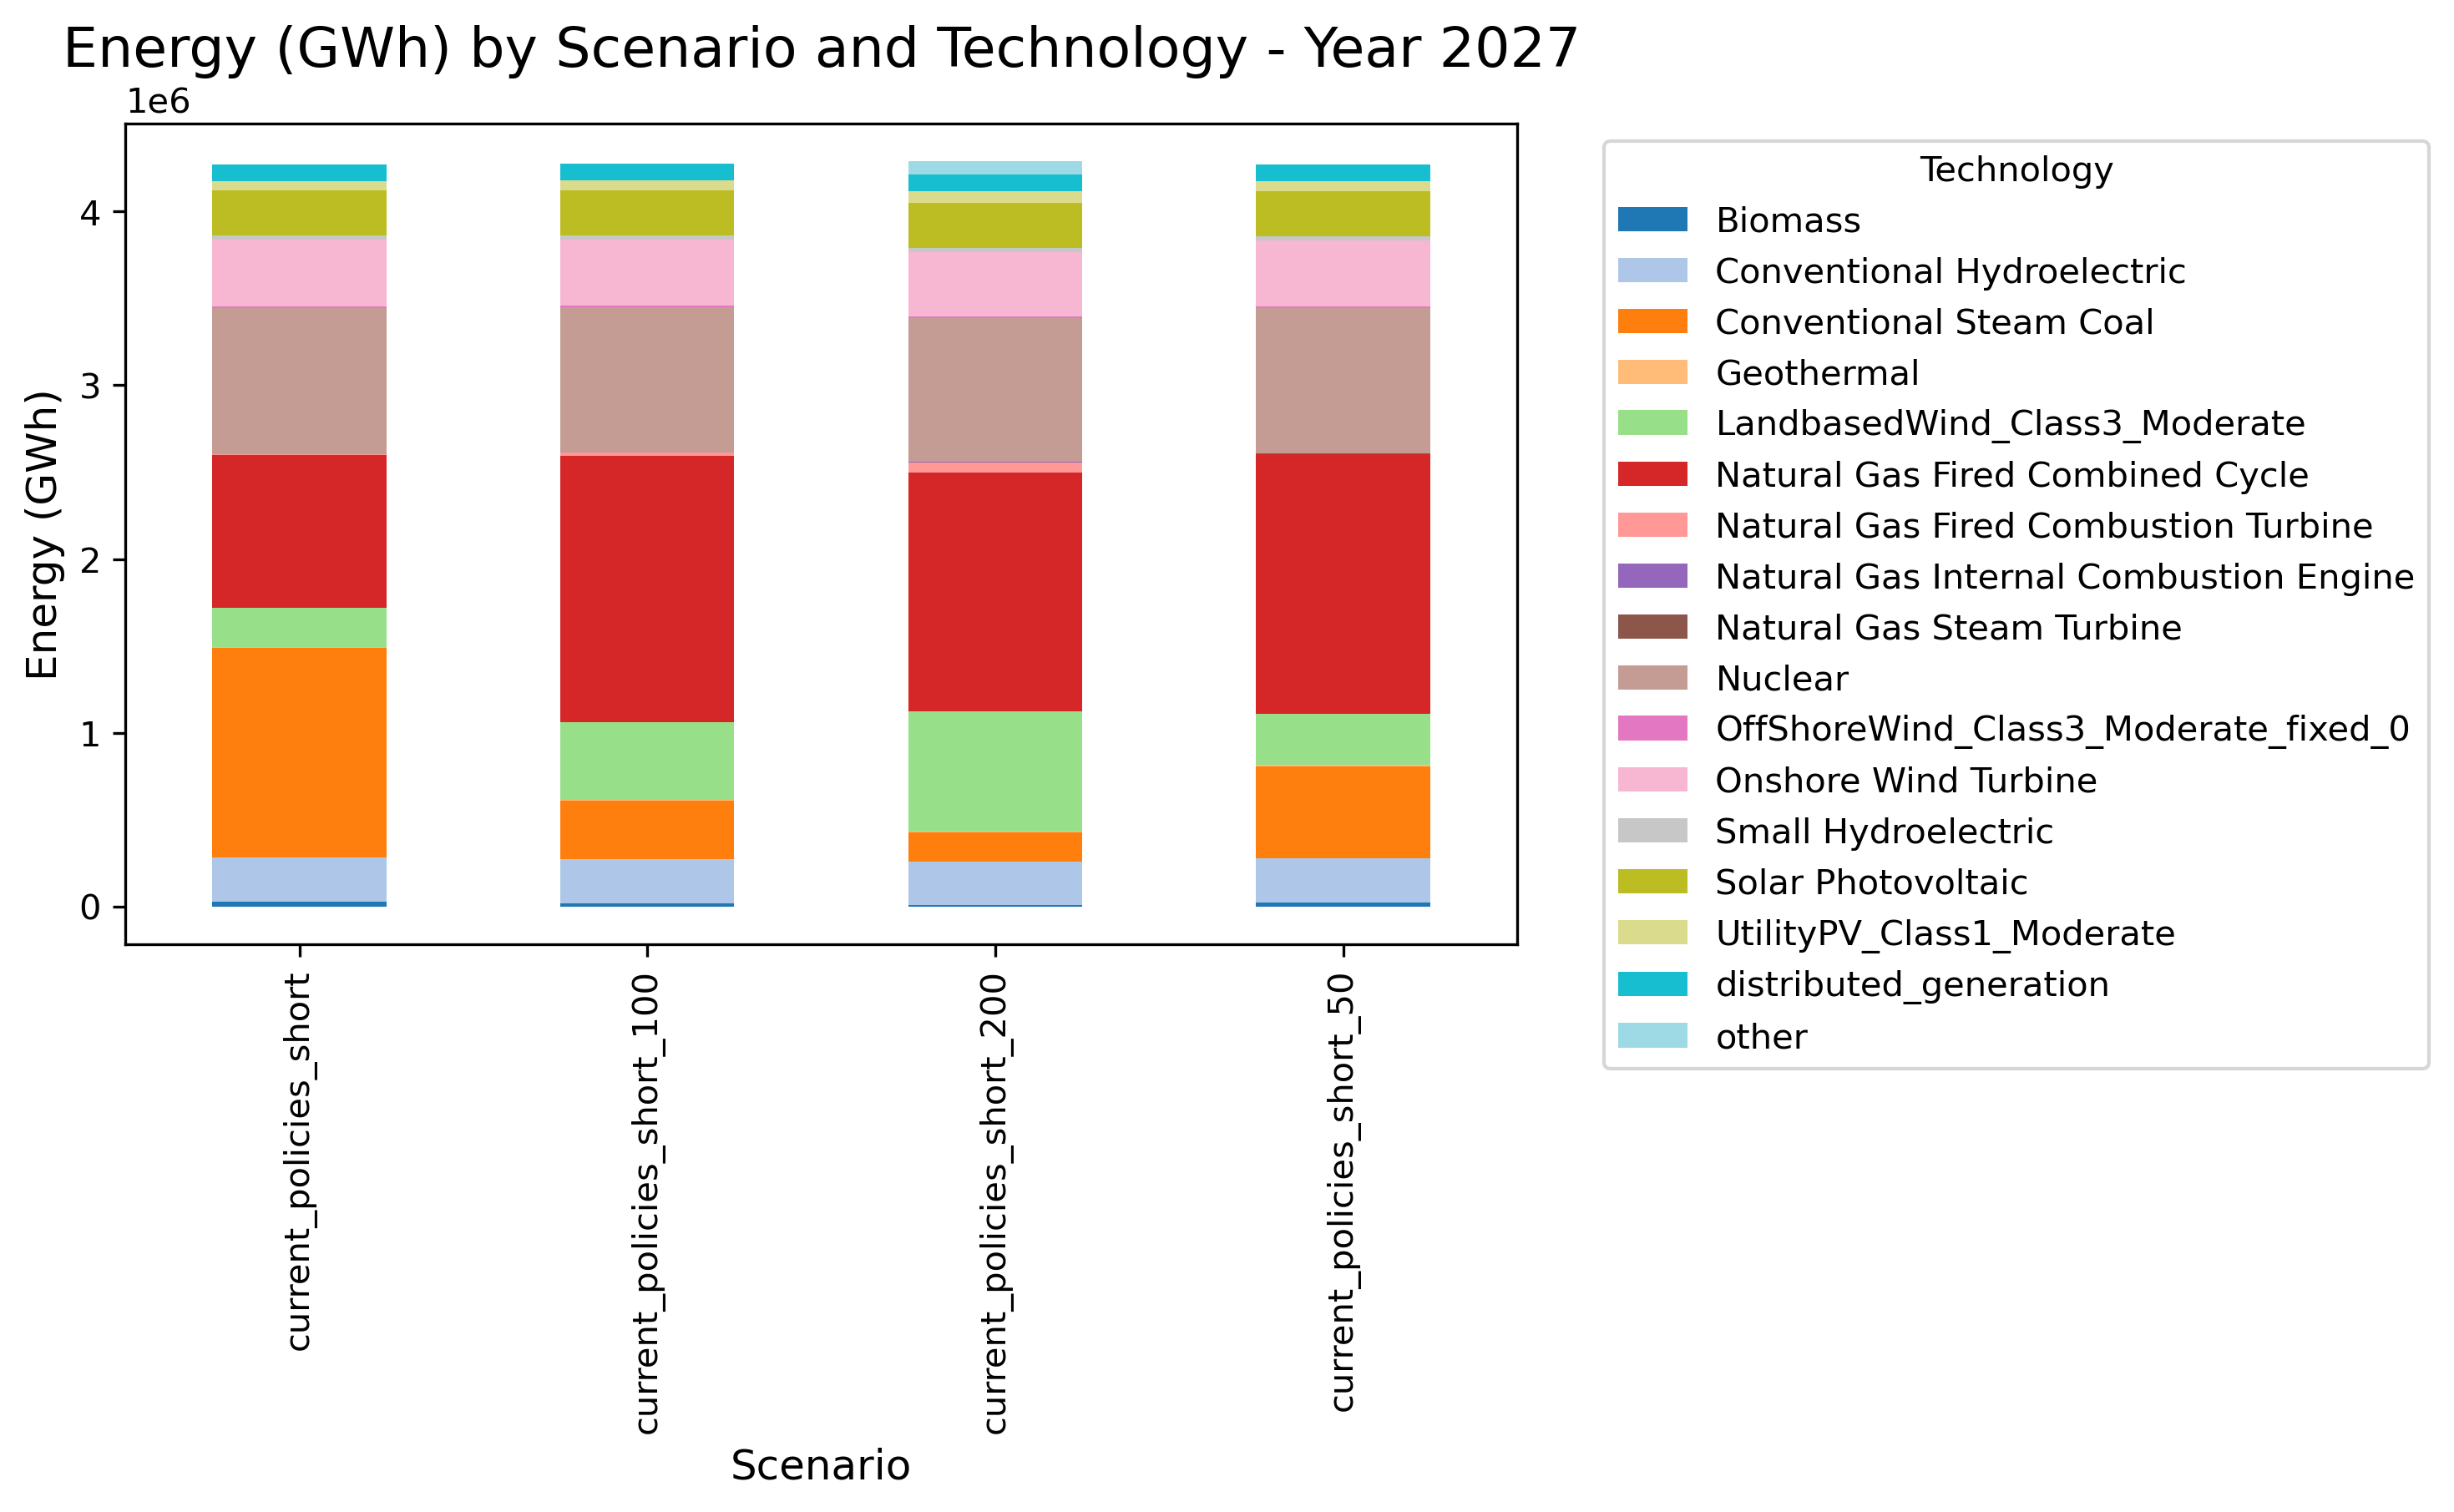
\includegraphics[width=0.45\textwidth]{Figures/EndogenousResults/current_policies_short/Dispatch_Relative_by_scenario_2027.png}}
    \subcaptionbox{2030}{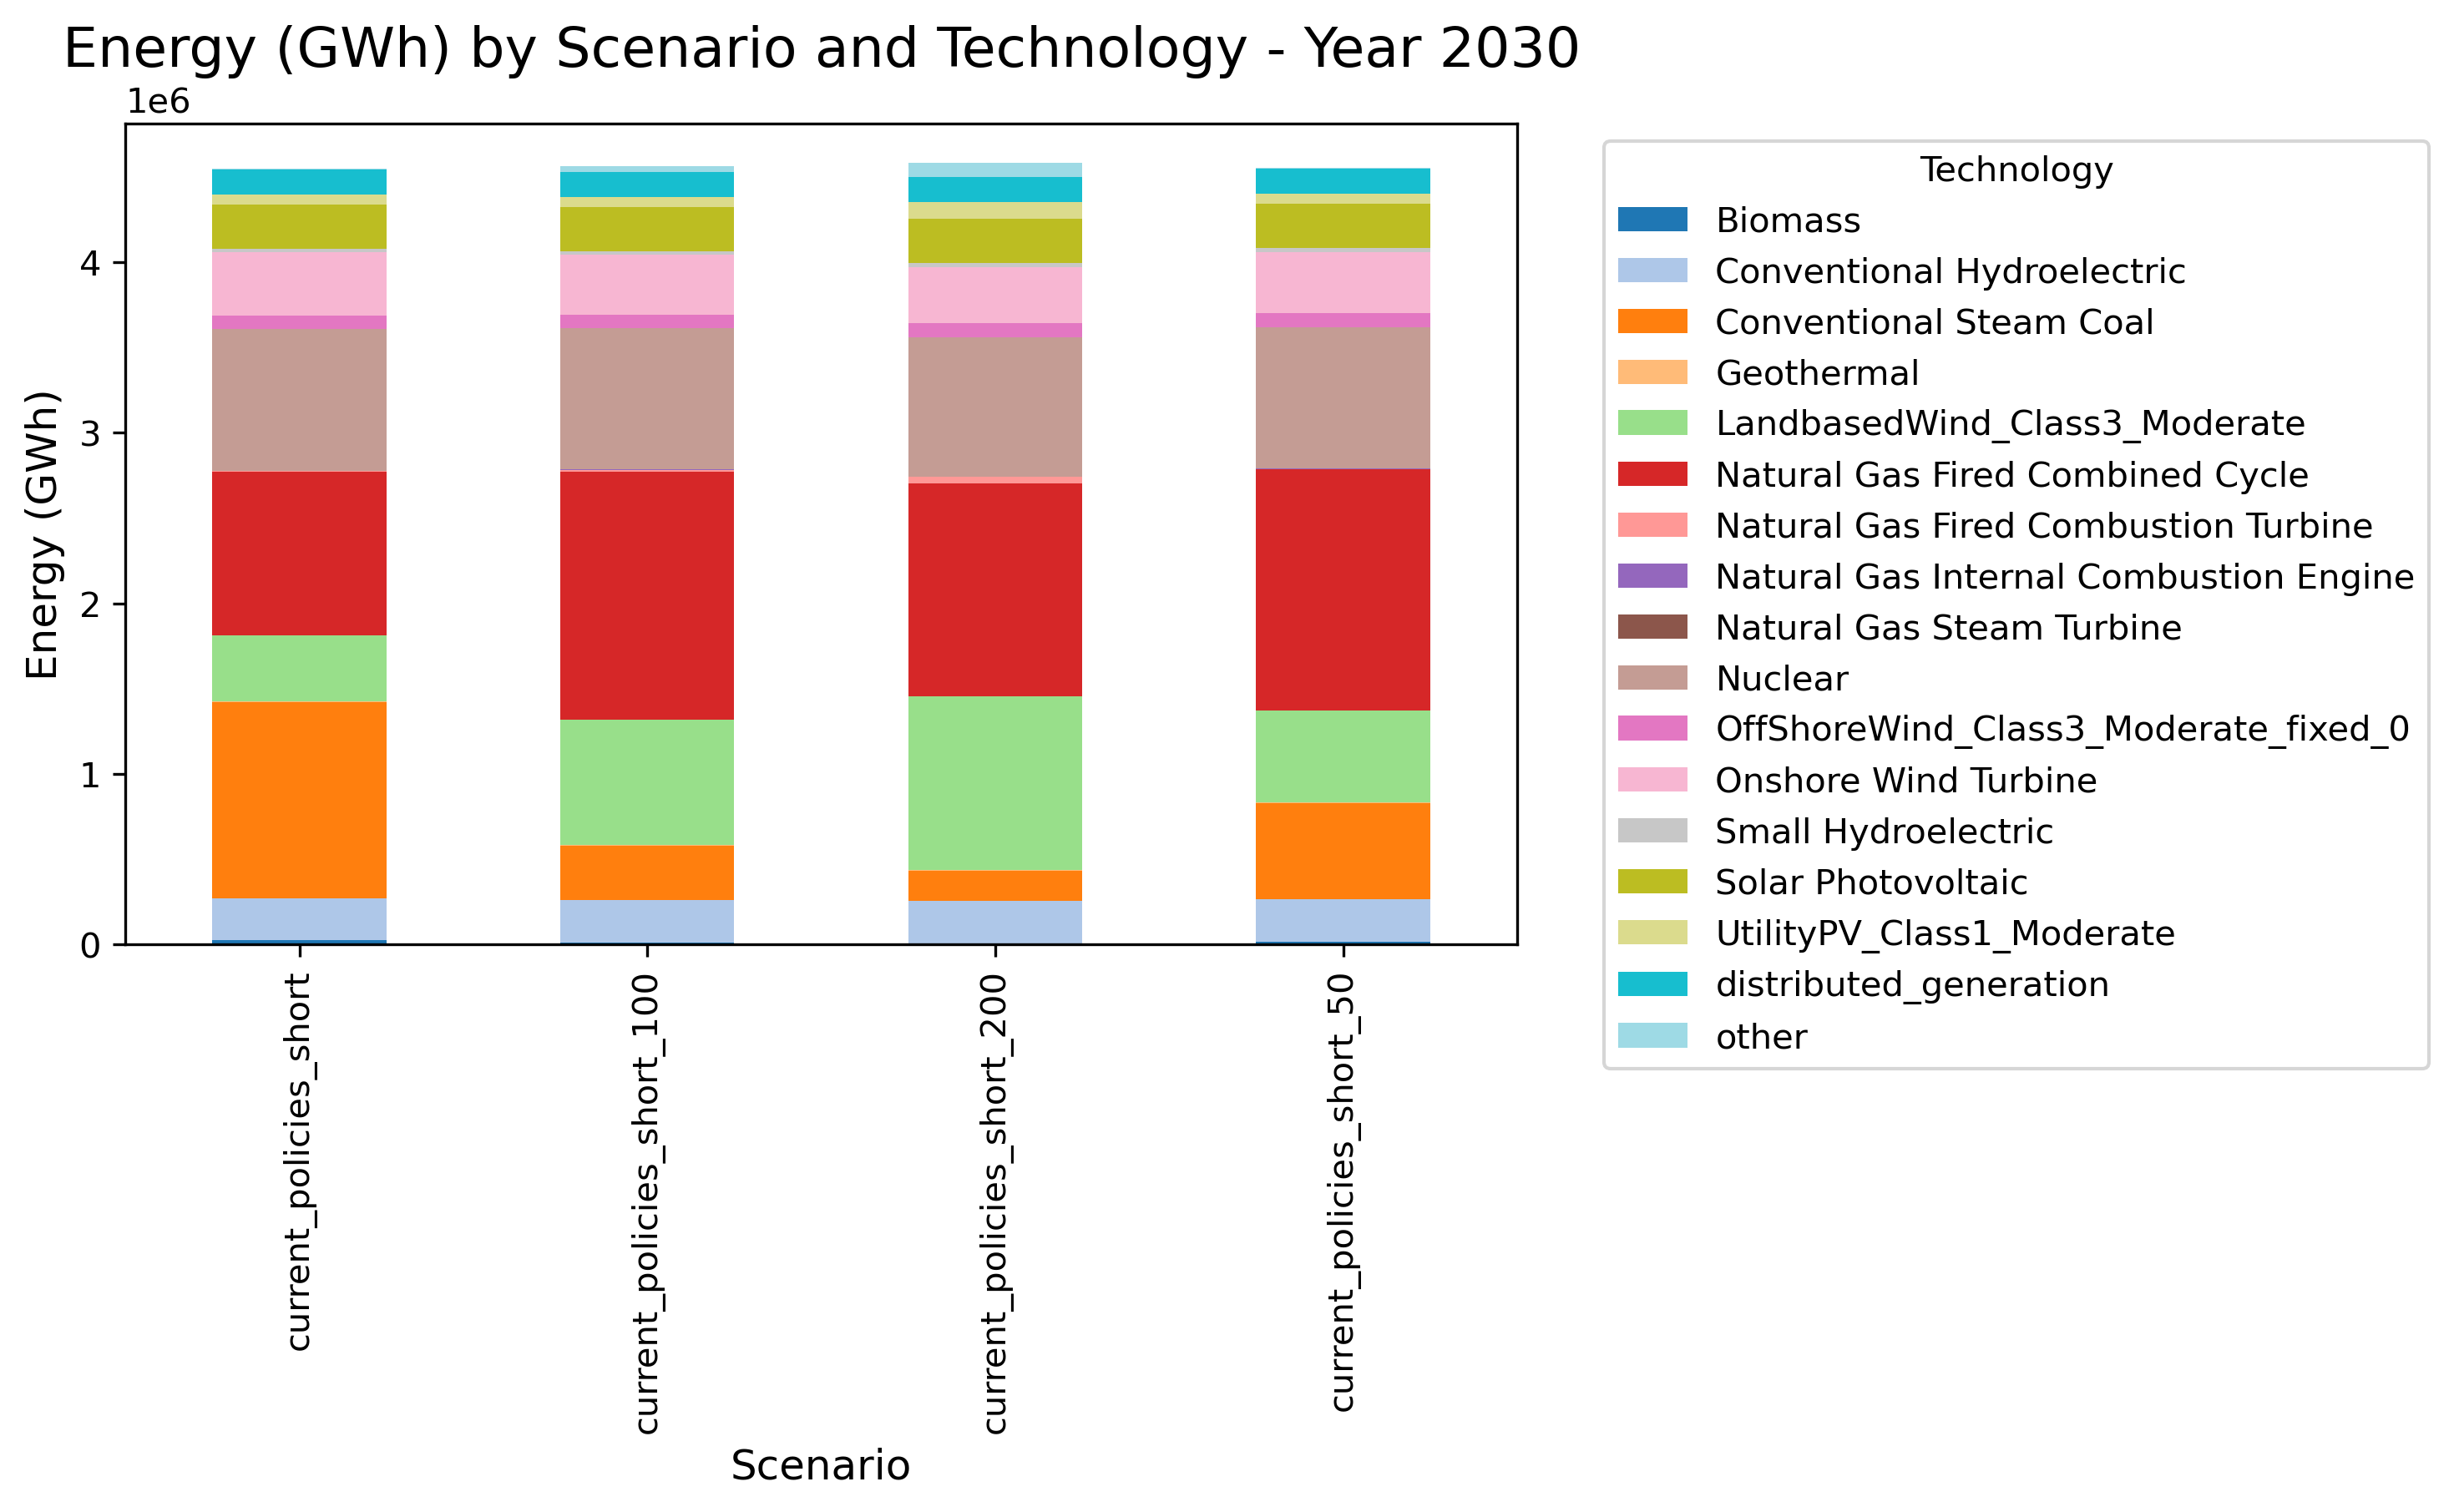
\includegraphics[width=0.45\textwidth]{Figures/EndogenousResults/current_policies_short/Dispatch_Relative_by_scenario_2030.png}}\\
    \subcaptionbox{2035}{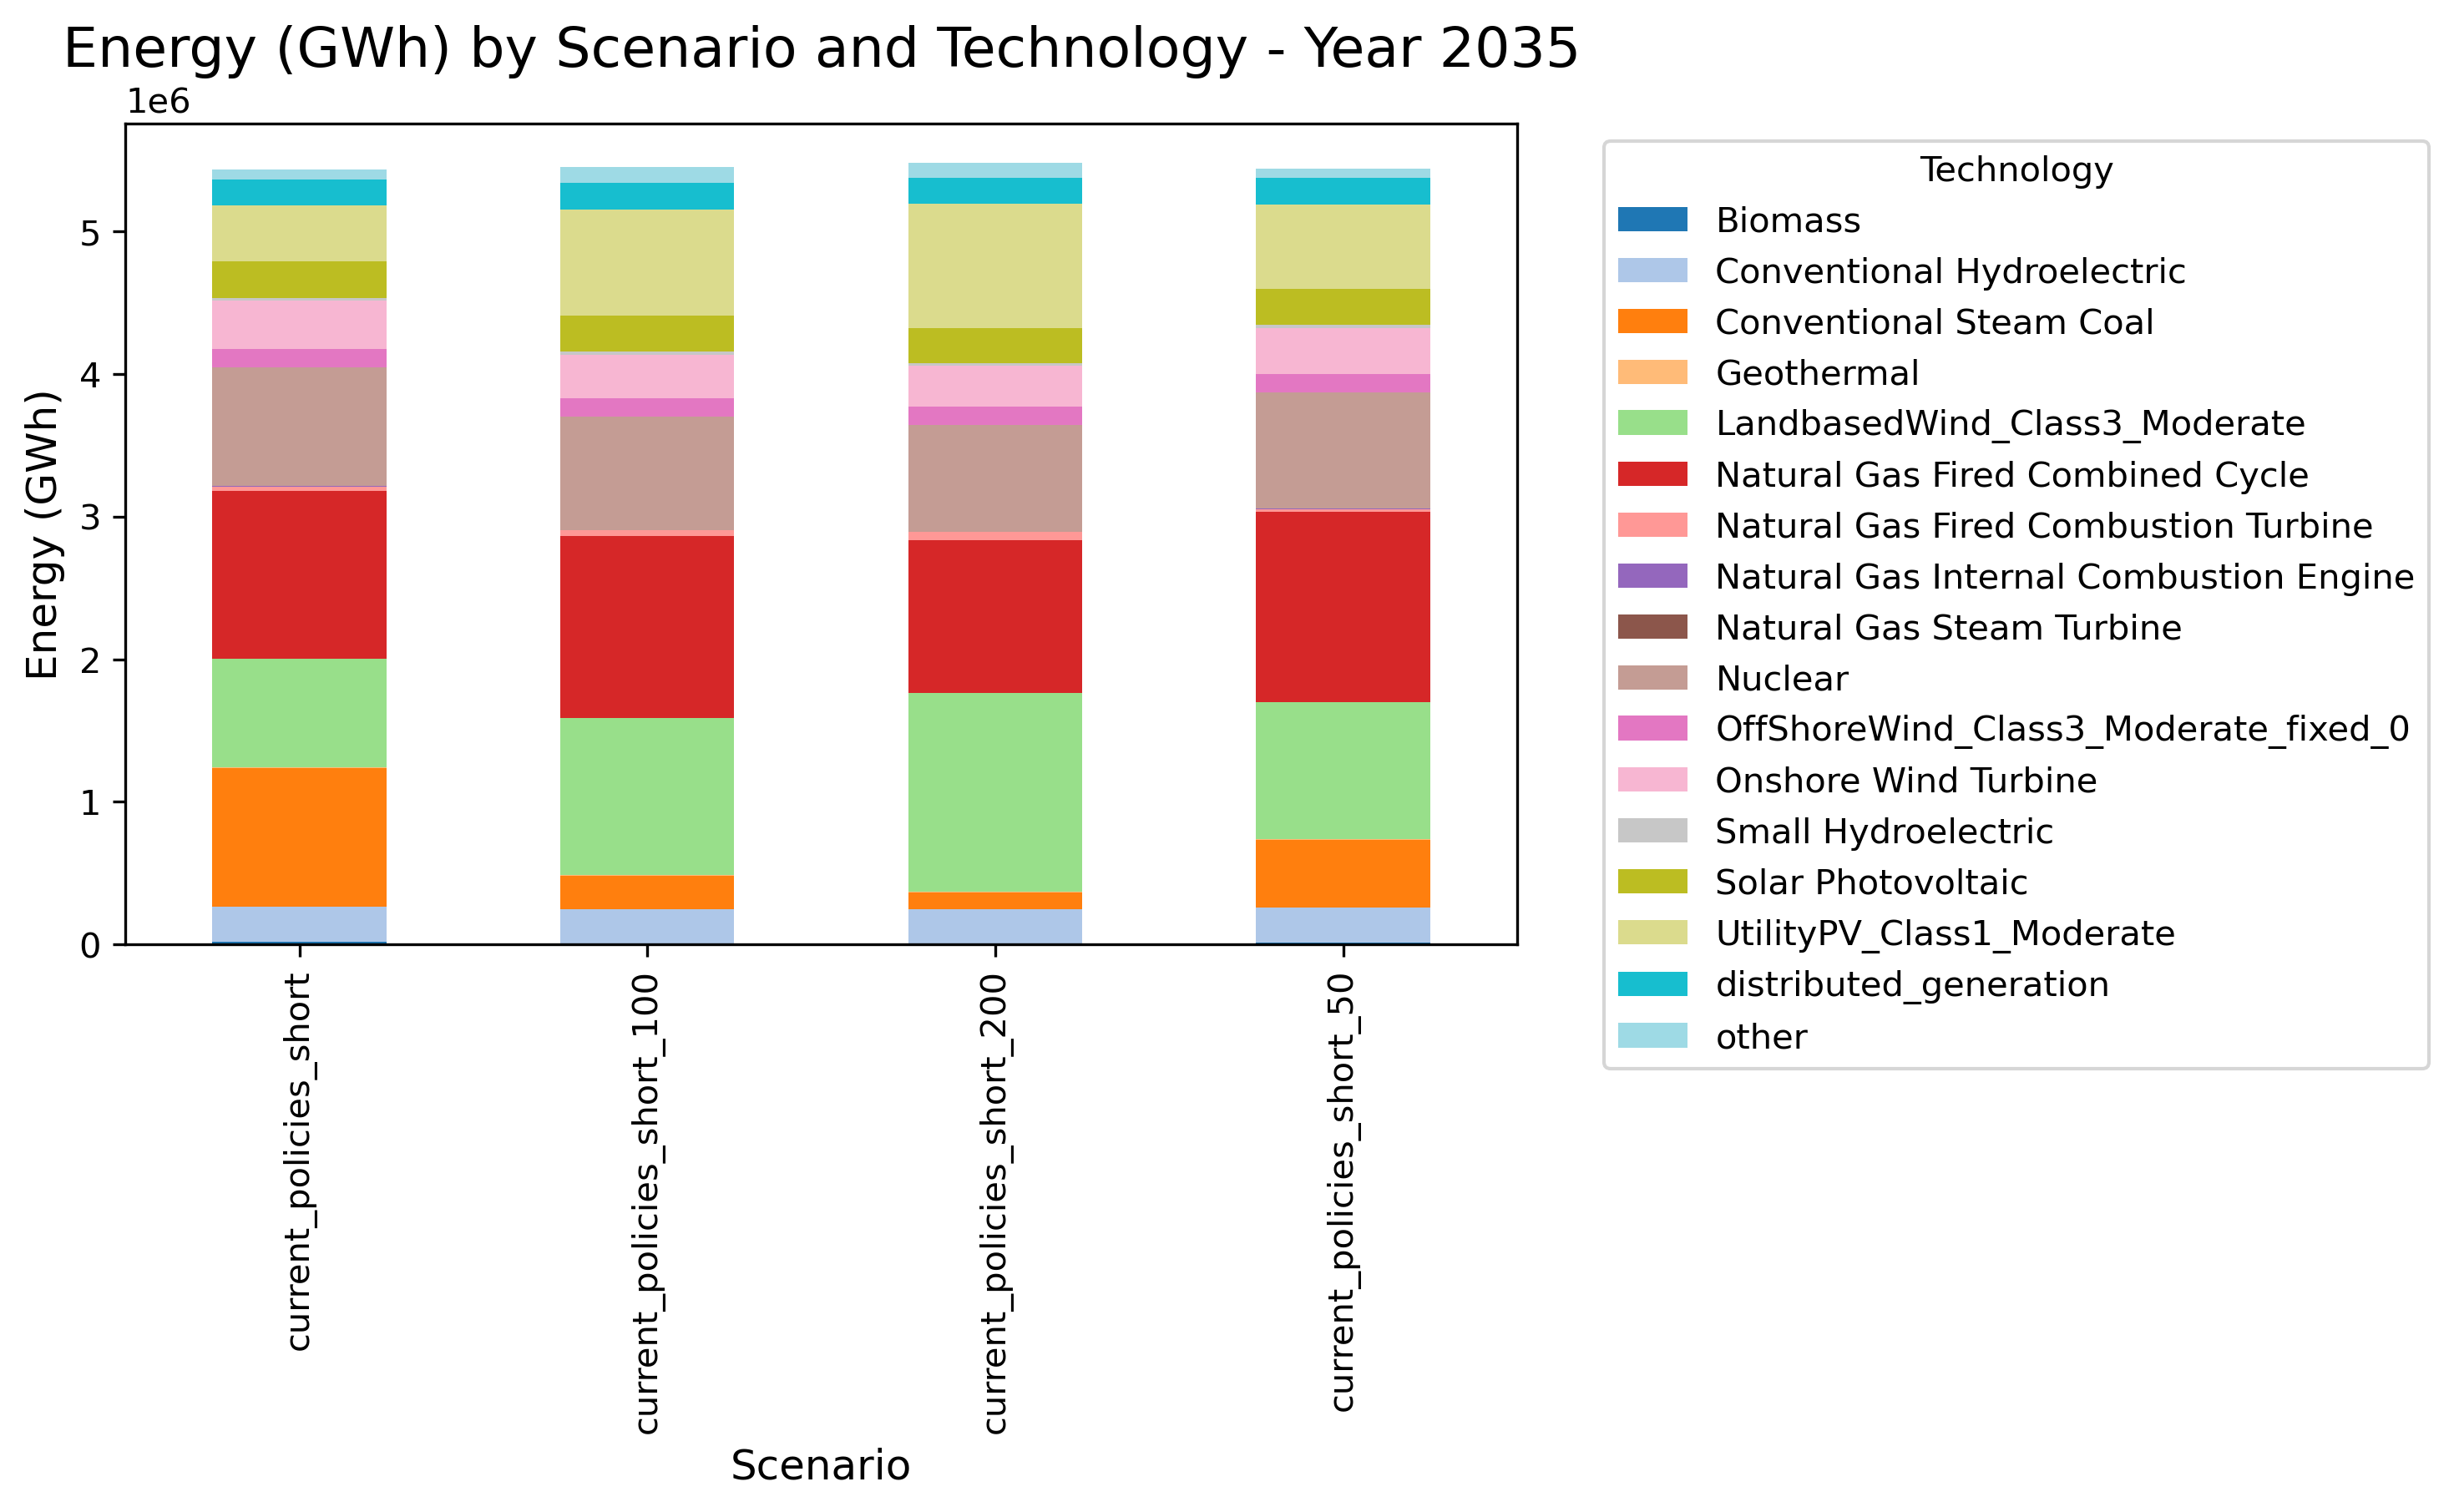
\includegraphics[width=0.45\textwidth]{Figures/EndogenousResults/current_policies_short/Dispatch_Relative_by_scenario_2035.png}}
    \subcaptionbox{2040}{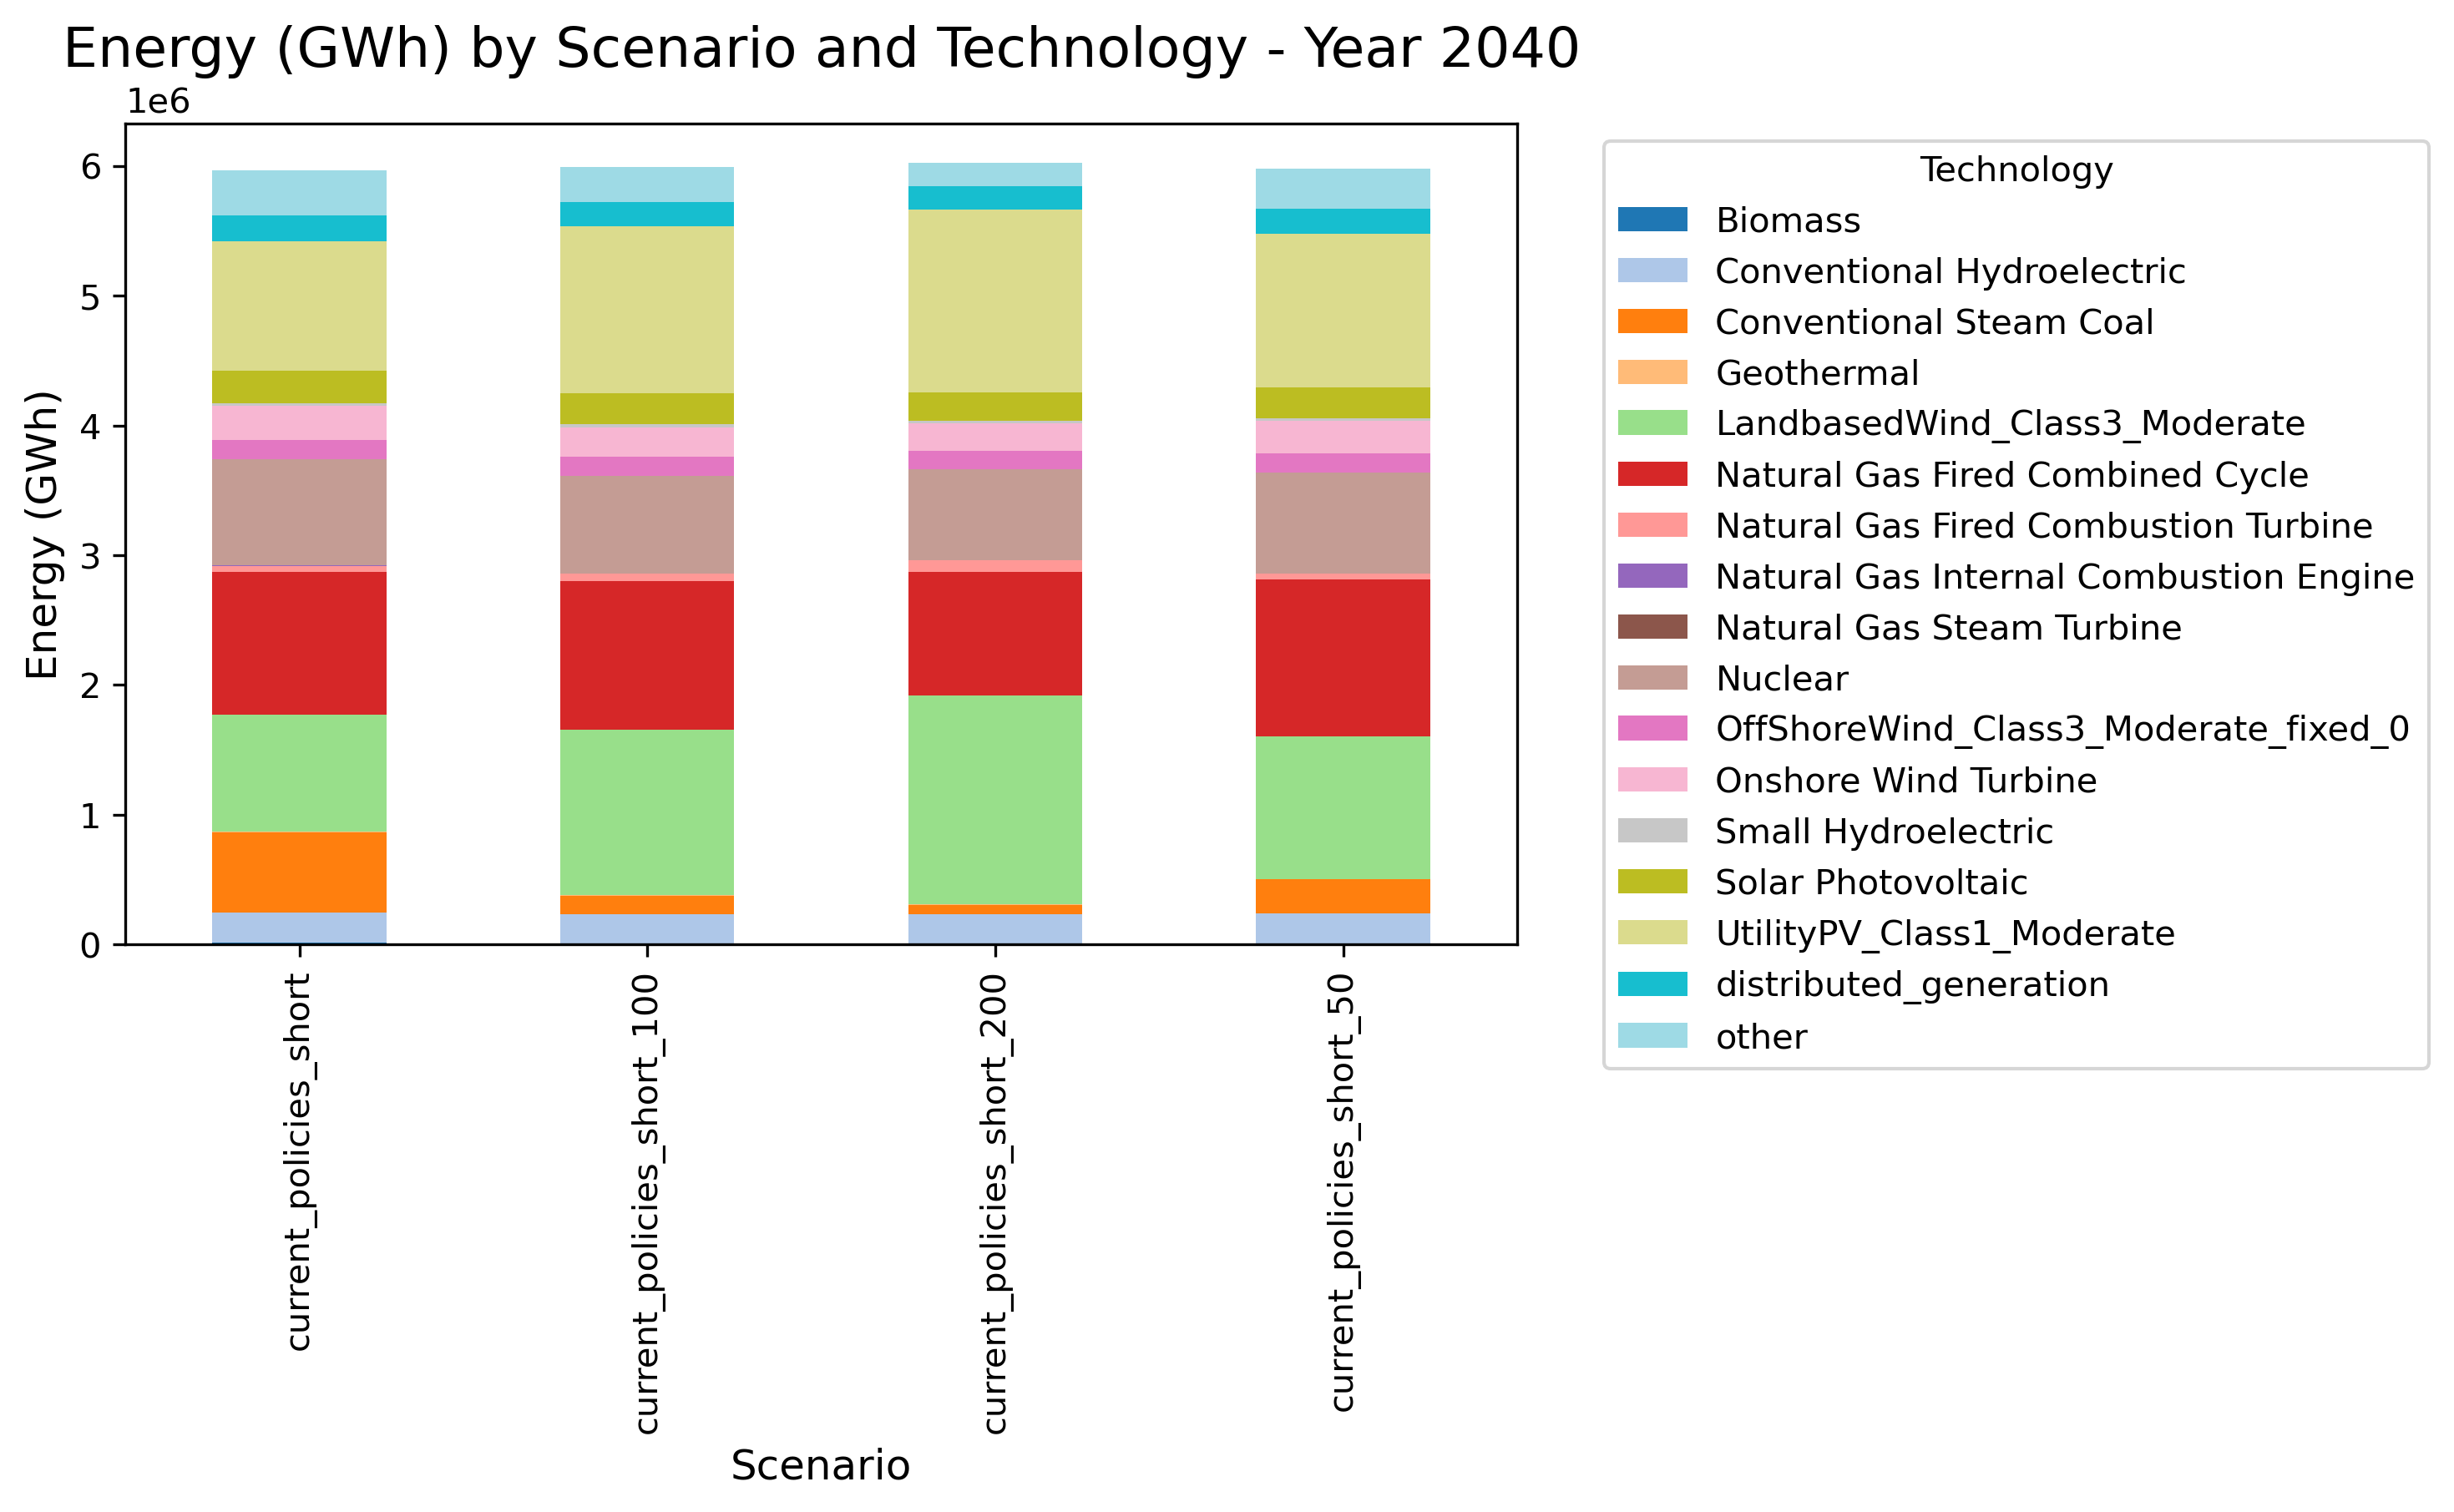
\includegraphics[width=0.45\textwidth]{Figures/EndogenousResults/current_policies_short/Dispatch_Relative_by_scenario_2040.png}}\\
    \subcaptionbox{2045}{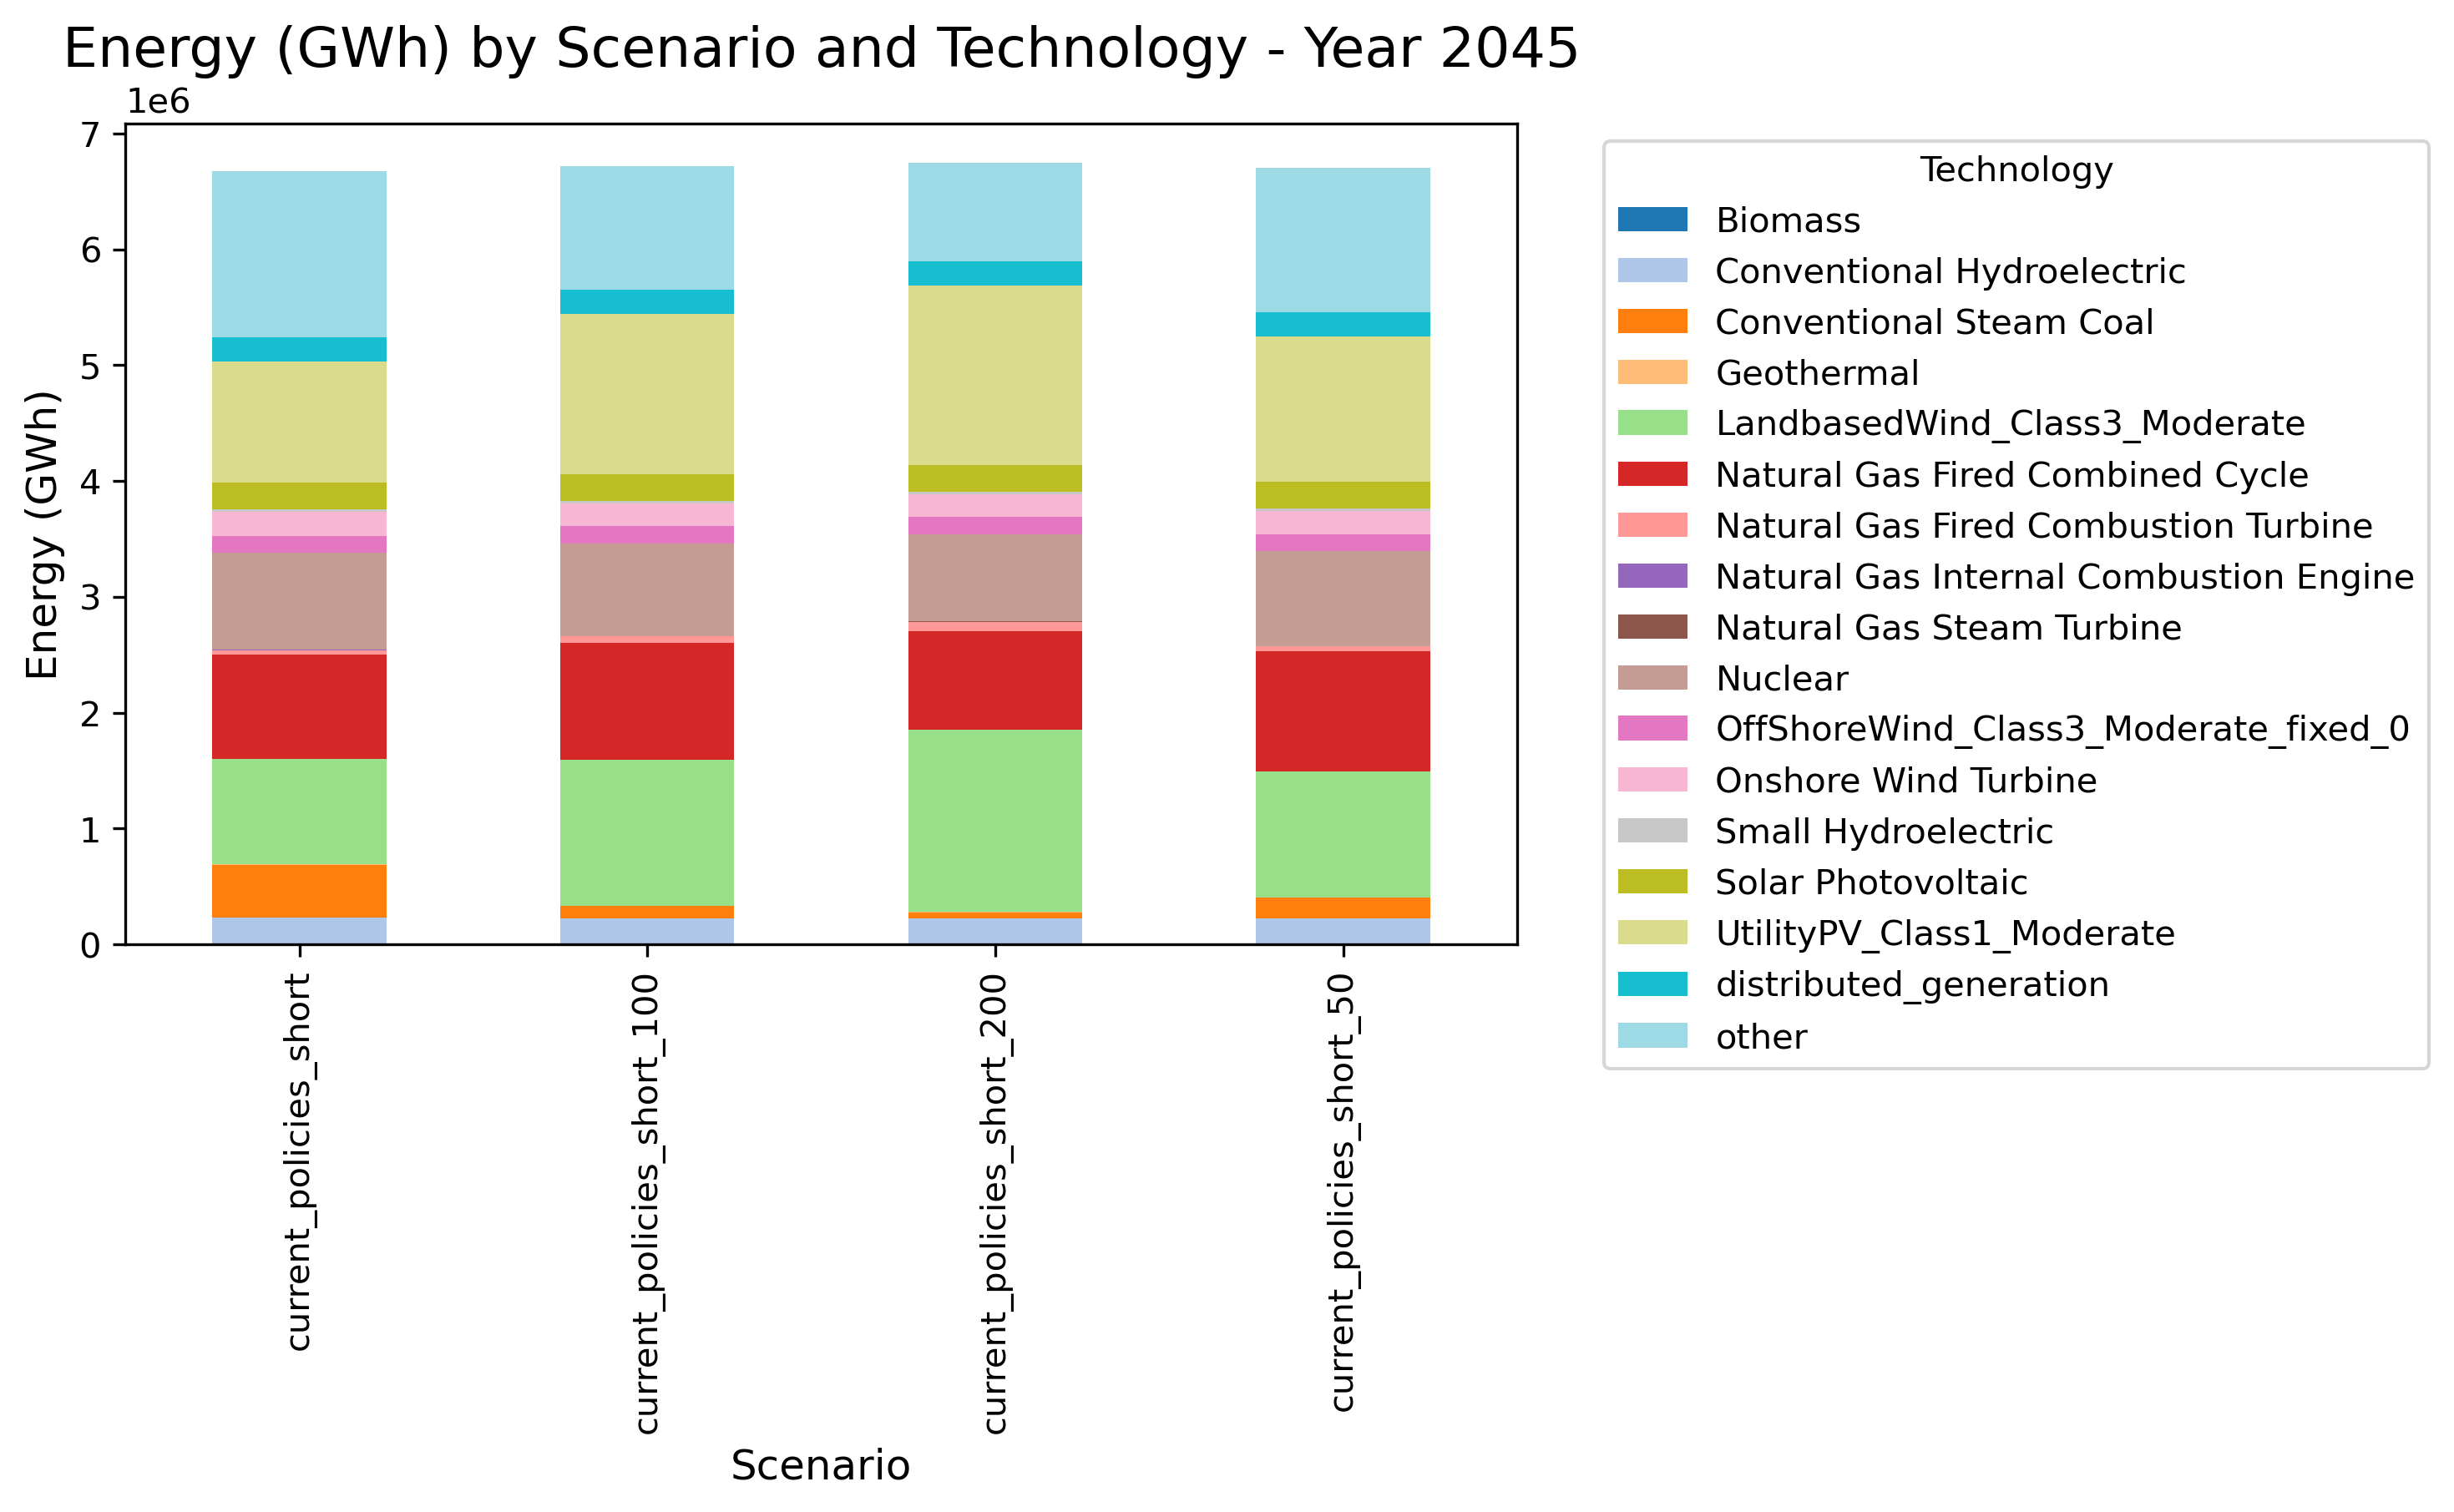
\includegraphics[width=0.45\textwidth]{Figures/EndogenousResults/current_policies_short/Dispatch_Relative_by_scenario_2045.png}}
    \subcaptionbox{2050}{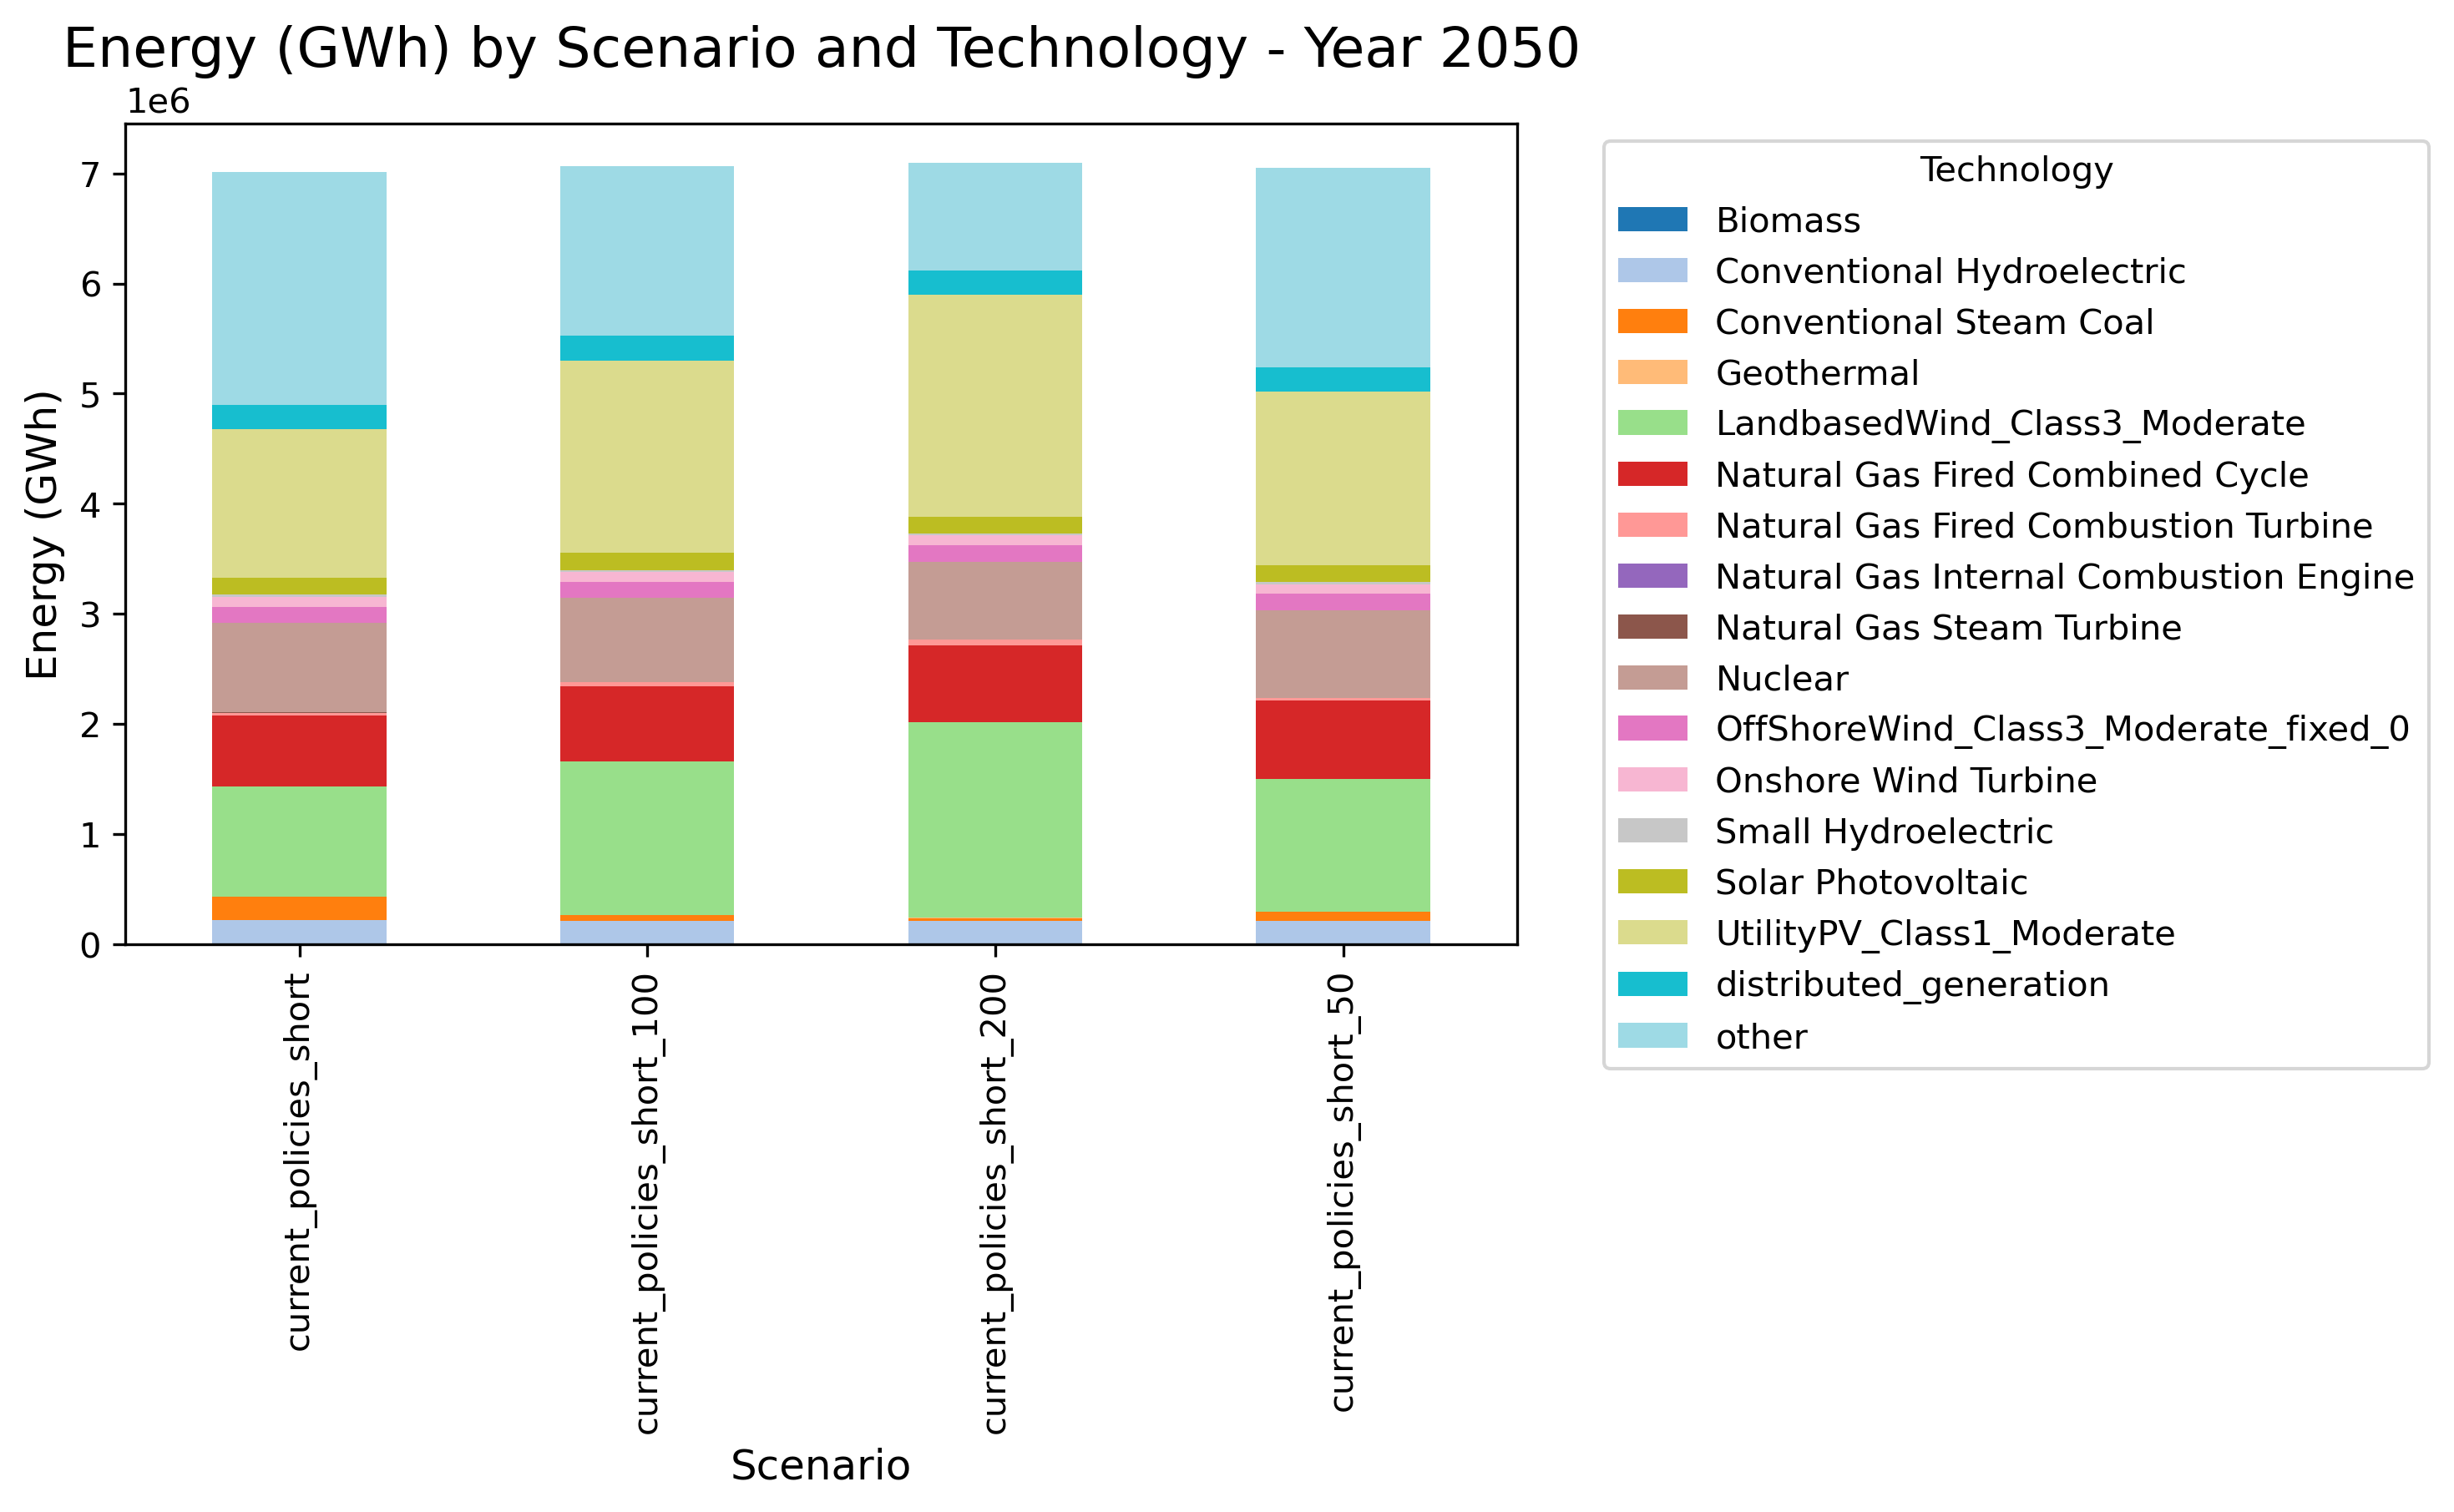
\includegraphics[width=0.45\textwidth]{Figures/EndogenousResults/current_policies_short/Dispatch_Relative_by_scenario_2050.png}}\\
    \caption{Generation by Technology by Scenario}
\end{figure}

\begin{figure}
    \centering
    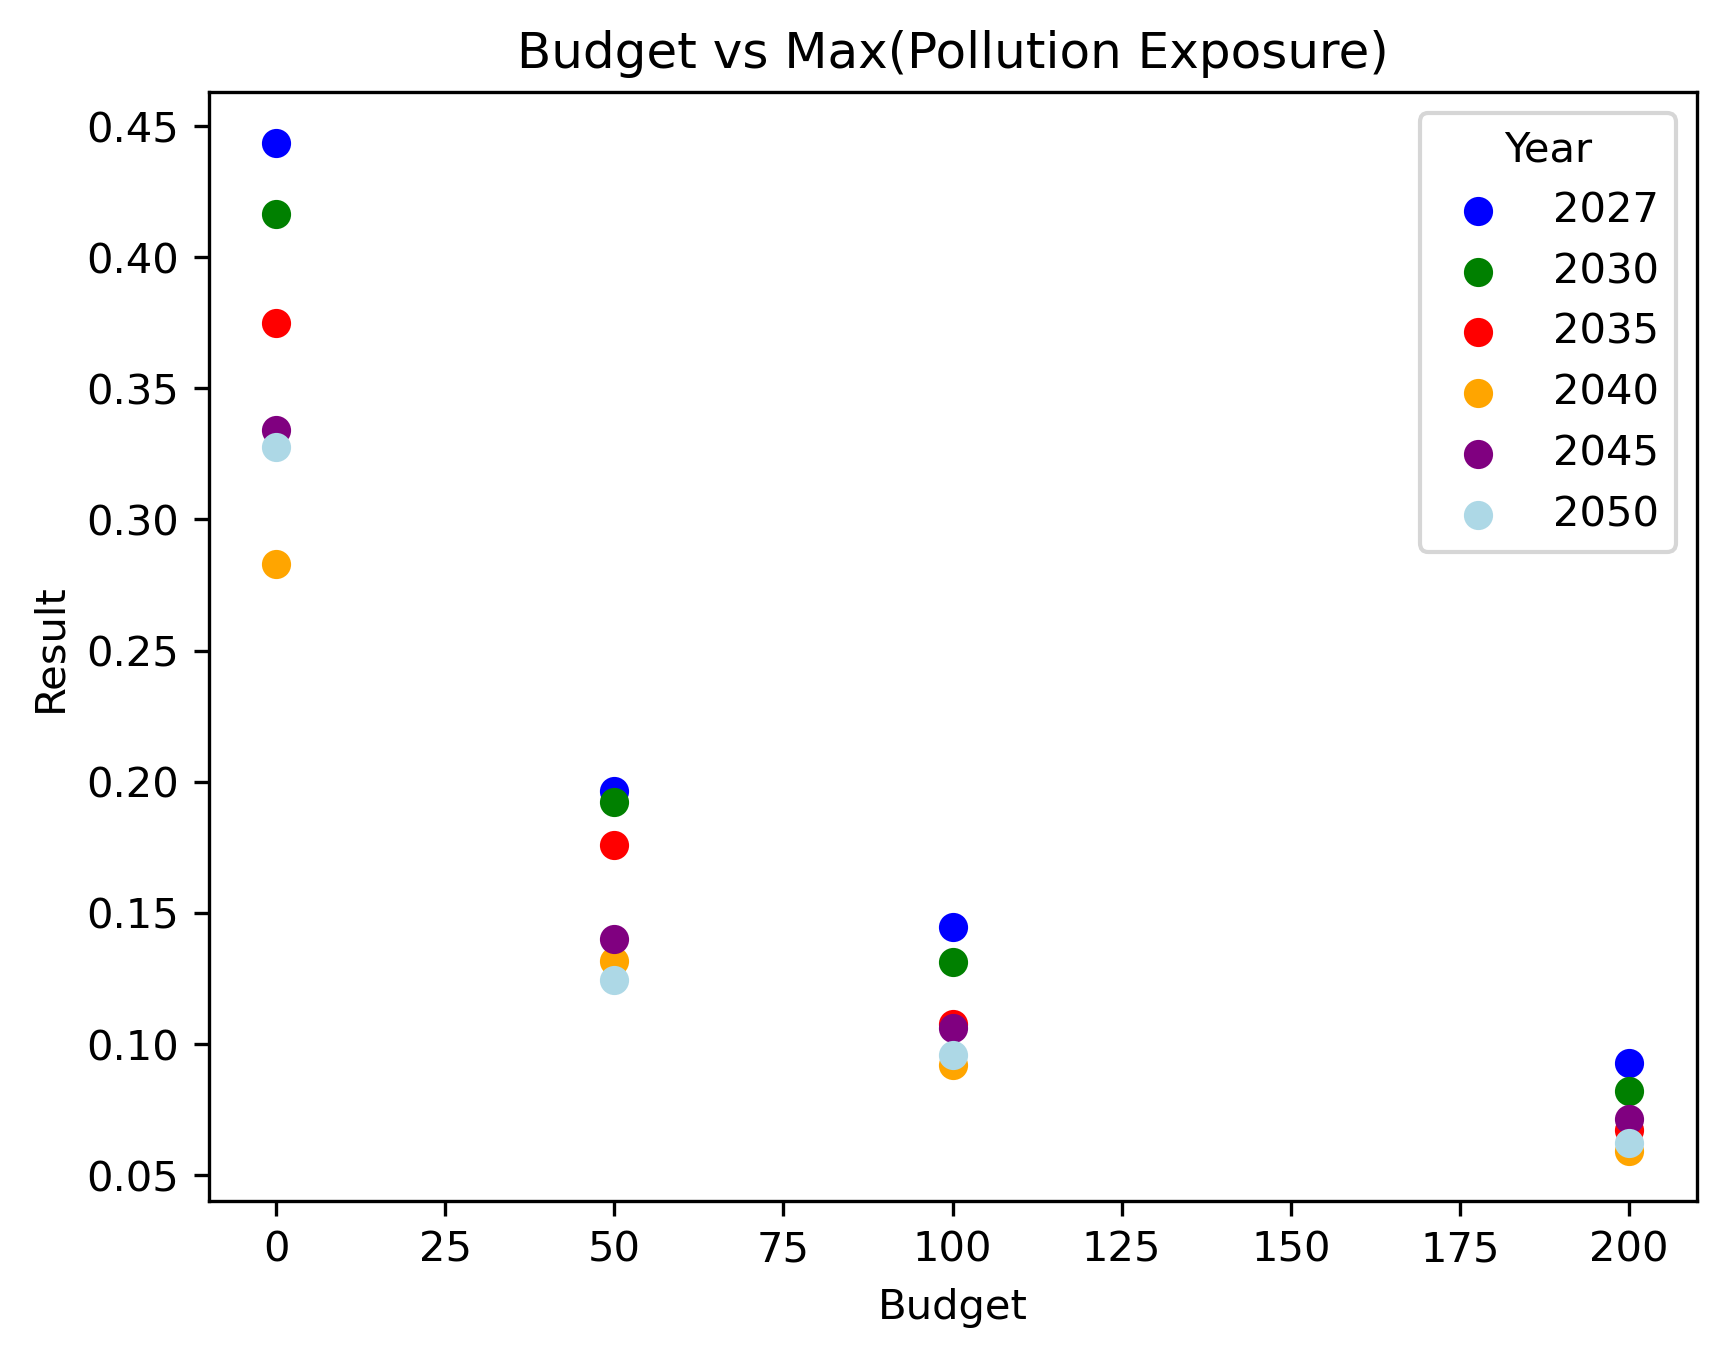
\includegraphics[width=0.7\linewidth]{Figures/EndogenousResults/current_policies_short/exposure_cost_PPF.png}
    \caption{Here we show the relationship between the objective function (min-max of exposure) and the cost limit constraint.}
    \label{PPF}
\end{figure}

\subsection{Comparison with carbon-only cuts}
While we think these results have important policy implications, namely that improving air quality equitably can happen at low costs, it's important to note that our results don't point to which policies would achieve the optimal solution. Rather, these results are prescriptive -- \textit{"Build X, Y, and Z in regions A,B, and C to achieve the deepest equitable cuts in air pollution at a certain cost."} 

Previous papers have found that carbon policies tend to decrease both total air pollution exposure, and the inequalities in air pollution exposure. This begs the question, how does a portfolio that minimizes air pollution exposure compare to a least-cost portfolio aimed at reducing carbon?

\section{Conclusion}
In this paper, we demonstrate how to endogenize air pollution exposure into a least-cost electricity planning model to create equitable reductions in air pollution burdens.    

While this method provides a map of how to produce equitable reductions in air pollution, it does not solve for what policies will get


\begin{singlespace}
\newpage
\bibliographystyle{jpe}
%\bibliographystyle{econometrica}
\bibliography{references.bib}
\end{singlespace}

\end{document}  